\section{Grundbegriffe}
\begin{def*}[note = Graph , index = Graph]
Graph $G = (V,E)$ \\
$V$ Menge, $0 < |V| < \infty$ (Knoten) \\
$E$ Relation auf $V, E \subseteq V^2$ (Kanten) \\
$G$ \textbf{ungerichtet}\index{Graph!ungerichtet}, falls $(u,v) \in E \iff (v,u) \in E$\\
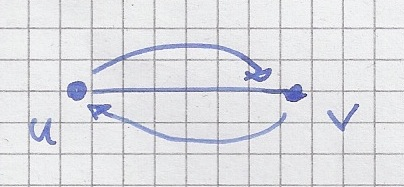
\includegraphics{Bild33} \\
Man schribt manchmal für ungerichtete $E \subseteq \{ \{u,v\} | u \neq v \}$\\
$\Gamma(v) \coloneqq \{ w \in V | (v,w) \in E \}$ \textbf{Nachbarschaft}\index{Nachbarschaft} \\
$\deg^-(v):$ Eingangsgrad\index{Grad!Eingangsgrad} \\
$\deg^+(v):$ Ausgangsgrad\index{Grad!Ausgangsgrad} \\
\[ \sum_N \deg^-(v) = \sum_N \deg^+(v) = |E| \]
Ungerichtet:
\[ \sum_N \deg(v) = 2|E| \]
$G$ \textbf{einfach}\index{Graph!einfach}, falls es keine \textbf{Loops} und keine \textbf{Mehrfachkanten}.
\end{def*}

\subsubsection{Grundbegriffe für einfache ungerichtete Graphen}
\begin{def*}[note = Weg , index = Weg]
$W = ( v_0 , \dotsc , v_l ) ; (v_i,v_{i+1}) \in E \quad \forall i = 0 , \dotsc , l-1$ (auch $v_0$-$v_l$-Weg ) $(l > 0)$
\end{def*}
\begin{def*}[note = Pfad , index = Pfad]
Weg, bei dem alle Knoten paarweise verschieden sind. ($v_0$-$v_l$-Pfad )
\end{def*}
\begin{def*}[note = zusammenhängend , index = Graph!zusammenhängend]
	$G=(V,E)$ zusammenhängend, falls $\forall u , v \in V \exists u$-$v$-Pfad
\end{def*}
\begin{def*}[note = Kreis , index = Kreis]
	$C=(v_1 , \dotsc , v_l)$, paarweise verschieden, $(v_i,v_{i+1}) \in E \forall i = 1 , \dotsc , l-1 \wedge (v_l , v_1) \in E \quad (l \geq 3 )$
\end{def*}
\begin{def*}[note = Teilgraph , index = Teilgraph]
	$H=(V',E')$ Teilgraph von $G=(V,E)$ falls $V' \subseteq V$ und $E' \subseteq V' \times V'$ und $E' \subseteq E$.
\end{def*}
\begin{def*}[note = induzierter Teilgraph , index = Teilgraph!induzierter]
	$H'$ von $V'$ induzierte Teilgraph, falls $\forall u , v \in V' : (u,v) \in E \implies (u,v) \in E'$. Wir schreiben $H'=G[V']$
\end{def*}
\begin{def*}[note = Zusammenhangskomponente , index = Zusammenhangskomponente]
	$G=(V,E) , (V_i)$ Partition von $V$ so, dass $\exists u$-$v$-Pfad $\iff \exists i : u \in V_i \ni v$. Dann $G[V_i]$ Zusammenhangskomponente von $G$.
\end{def*}
\begin{def*}[note = Brücke , index = Brücke]
	$e \in E$ Brücke falls $G'=(V,E \setminus \{e\})$ eine Zusammenhangskomponente mehr hat als $G$.
\end{def*}
\begin{satz*}
	$G=(V,E)$ hat mindestens $|V|-|E|$ Zusammenhangskomponenten
	\begin{bew}
		$G=(V,\varnothing)$ hat |V| Zusammenhangskomponenten. Jede Kante $e$, diehinzugefügt wird, reduziert ihre Anzahl höchstens um $1$.
	\end{bew}
	\begin{korr*}
		$G$ zusammenhängend $\implies |V| - |E| \leq 1$
	\end{korr*}
\end{satz*}